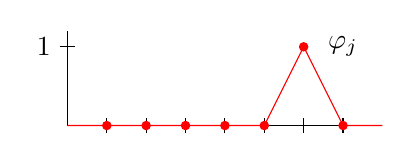
\begin{tikzpicture}[scale=1]
	%\fill[black!20!white] (2.15,0) -- ++(0,0.35) -- ++(0.65,0.26) -- ++(0,-0.61) -- cycle;
	%\draw (2.15,0) 
	\draw (0,0) -- ++(0,1.2);
	\draw (0,0) -- ++(4,0);

	\draw[red] (0,0) -- ++(2.5,0) -- ++(0.5,1) -- ++(0.5,-1) -- ++(0.5,0);
	%\filldraw (2.15,0.35) circle (0.4pt);
	
	\draw (-0.1,1) -- ++(0.2,0);
	
	\draw (0.5,-0.1) -- ++(0,0.2);
	\draw (1  ,-0.1) -- ++(0,0.2);
	\draw (1.5,-0.1) -- ++(0,0.2);
	\draw (2  ,-0.1) -- ++(0,0.2);
	\draw (2.5,-0.1) -- ++(0,0.2);
	\draw (3  ,-0.1) -- ++(0,0.2);
	\draw (3.5,-0.1) -- ++(0,0.2);
	
	
	\filldraw[red] (0.5,0) circle (1.5pt);
	\filldraw[red] (1  ,0) circle (1.5pt);
	\filldraw[red] (1.5,0) circle (1.5pt);
	\filldraw[red] (2  ,0) circle (1.5pt);
	\filldraw[red] (2.5,0) circle (1.5pt);
	\filldraw[red] (3  ,1) circle (1.5pt);
	\filldraw[red] (3.5,0) circle (1.5pt);
	
	
	\node at (-0.3,1) {1};
	\node at (3.5,1) {$\varphi_j$};
	%\node at (2.8,-0.1) {b};
	%\node at (2.15,0.53) {f(a)};
	%\node at (2.77,0.71) {f(b)};
	
	\end{tikzpicture}